\section{Machine learning: random forest}
\label{chapter3_section8}


Random forests constitute a very popular algorithm in machine learning. They belong to the class of ensemble learning models, and rely on a simple principle: combine several weak regressors to construct a strong one. Their intuitiveness and efficiency make them very appealing models. The main algorithm is due to \cite{Breiman2001}, but variants exist, like the extra tree algorithm of \cite{Geurts2006}.


\subsection{Formulation}
\label{chapter3_section8_subsection1}


At the base of random forests are regression trees. A regression tree is a decion rule that maps a set of $p$  regressors $x = (x_1, x_2, \cdots, x_p)$ to a predicted value $\hat{y}$. To do so, The predictor space is segmented into a number $M$ of simple rectangular regions $R_1, \cdots, R_M$. This generates a set of splitting rules that can be summarized as a tree, the nodes of the tree corresponding to the decisions over feature values, and the terminal leafs corresponding to the terminal regions that provide the predicted values. This is illustrated in Figure \ref{fig_c3_s8_ss1_1}.

\begin{figure}[H]
\centering
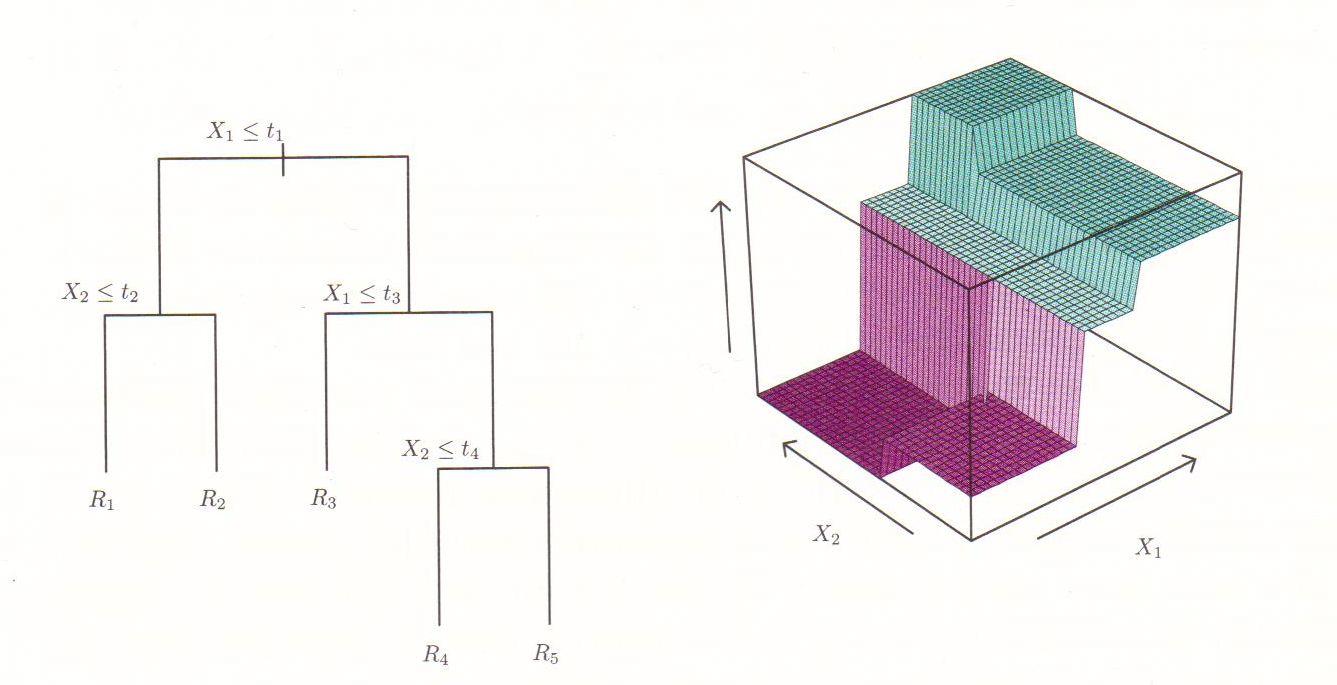
\includegraphics[scale=0.45]{images/regression_tree.png}
\caption{A regression tree with implied regression regions (credit: \cite{Gareth2013})}
\label{fig_c3_s8_ss1_1} 
\end{figure}

In mathematical terms, a regression tree can be formulated as a function of the form:

\begin{equation}
\hat{y} = f(x) = \sum_{m=1}^{M}{c_m \ . \ \ind(x \in R_m)}
\label{equation_c3_s8_ss1_1} 
\end{equation}

Regression trees tend to overfit. That is, they have low bias but high variance, which results in poor predictive performance out-of-sample. The random forest algorithm overcomes this issue by reducing the variance thanks to model averaging. The principle is simple: rather than using a single tree, use an ensemble of bootstrapped trees, and average their predictions. In addition, each bootstrapped tree is fit only a small subset of features. This allows to explore a larger portion of the feature space and to decorrelate the trees.

Formally, the random forest algorithm goes as follows:

\textbf{Algorithm 9: Random forest} \vspace{3mm} \\
1. Create a bootstrapped sample by randomly selecting $J$ observations (with replacement) over the $N$ available in the sample.

2. Fit a regression tree on this sample, but for each split considered, select randomly only a small number $q$ of features over the $p$ available. Set for instance $q=0.2 p$ or $q=\sqrt{p}$.

3. Repeat steps 1-2 a total number of $B$ times, fitting at each iteration the regression tree $f^b(x)$, for $b=1, \cdots, B$. 

4. Obtain finally the random forest predictor $f(x) = \frac{1}{B} \sum_{b=1}^{B}{f^b(x)}$.


\subsection{Estimation}
\label{chapter3_section8_subsection2}


Estimating a random forest amounts to fitting a set of regression trees. There exist several procedures to fit a regression tree,. A notorious one is the CART algorithm of \cite{Breiman1984}, a simple version of which can be found in \cite{Hastie2009}:

\newpage

\textbf{Algorithm 10: regression tree} \vspace{3mm} \\
1. Starting with all the data, consider a splitting features $j \in 1, \cdots, p$ and a split point $s$, and define the pair of half-planes: \\
$R_1(j,s) = \{x: x_j \leq s\}$ and $R_2(j,s) = \{x: x_j > s\}$.

2. Find the splitting feature $j$ and the split point $s$ that solve: \\
$\underset{j,s}{argmin} \left[ \mathlarger{\sum}\limits_{x_i \in R_1(j,s)} (y_i - \bar{y}_{R_1})^2 + \mathlarger{\sum}\limits_{x_i \in R_2(j,s)} (y_i - \bar{y}_{R_2})^2 \right]$ \\
where $\bar{y}_{R_1}$ and $\bar{y}_{R_1}$ respectively denote the means for the observations in $R_1(j,s)$ and $R_2(j,s)$.

3. repeat the process over the resulting regions, and stop when some termination criterion is reached. Such criterion include a maximum tree depth, a mximum number of leaves, or a minimum number of observations per leaf.



\subsection{Prediction}
\label{chapter3_section8_subsection3}


Prediction is perfectly trivial with random forests and follows from direct application of the model. Given a vector of regressors $x$, the prediction $\hat{y}$ is given by:

\begin{equation}
\hat{y} = f(x) = \frac{1}{B} \sum_{b=1}^{B}{f^b(x)}
\label{equation_c3_s8_ss3_1} 
\end{equation}


\subsection{Application}
\label{chapter3_section8_subsection4}

A useful aspect of random forests is that they permit to calculate what is known as variable importance. A feature $x_j$ is important for the model if breaking the link between this feature and the target $y$ significantly increases the prediction error. Formally, define by $\bar{x}^b$ the set of observations not selected by the bootstrap at iteration $b$ of the random forest algorithm, and denote by $\bar{x}_p^b$ a copy of this set where a random permutation is applied to $x_j$. Denote respectively by $L(\bar{x}^b)$ and $L(\bar{x}_p^b)$ the mean squared errors obtained on the non-permuted and permuted datasets. If $x_j$ is important, then randomly permuting it should deteriorate the predictions. 

Therefore, one can measure the importance of $x_j$ from:

\begin{equation}
I(x_j) = \frac{1}{B} \sum_{b=1}^{B}{L(\bar{x}_p^b) - L(\bar{x}^b)}
\label{equation_c3_s8_ss4_1} 
\end{equation}

As a first application, Figure \ref{fig_c3_s8_ss4_1} plots the variable importance of the project dataset for the prediction of real GDP growth. The model predicts GDP on two lags of each feature.

\begin{figure}[H]
\centering
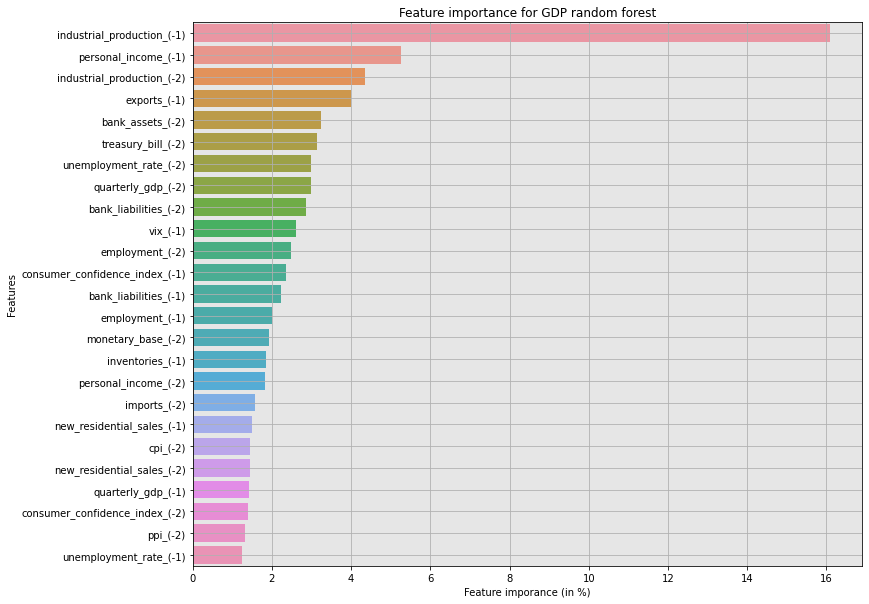
\includegraphics[scale=0.5]{images/variable_importance.png}
\caption{Variable importance in the prediction of GDP growth}
\label{fig_c3_s8_ss4_1} \vspace{-3mm}
\end{figure}

More than 20\% of the importance goes to one variable: industrial production. This is hardly surprising as industrial production represents a proxy for national production, so the correlation with GDP is high. The other important features are closely related to short-term activity and fluctuations, which once again makes sense for immediate predictions of GDP: exports and imports, employment and unemployment rate, consumer confidence index, inventories. Interestingly enough, a few financial variables also seem to help predict GDP: bank assets and liabilities, treasury bill and the VIX. The main point however is that past values of GDP contribute only moderately to nowcast GDP (about 5\%). This stresses the domination of high frequency predictors over past values of low frequency variables, the former carrying more recent and valuable information.

It is also interesting to investigate which features determine the others within the dataset. This is shown in Figure \ref{fig_c3_s8_ss4_2}.

\begin{figure}[H]
\centering
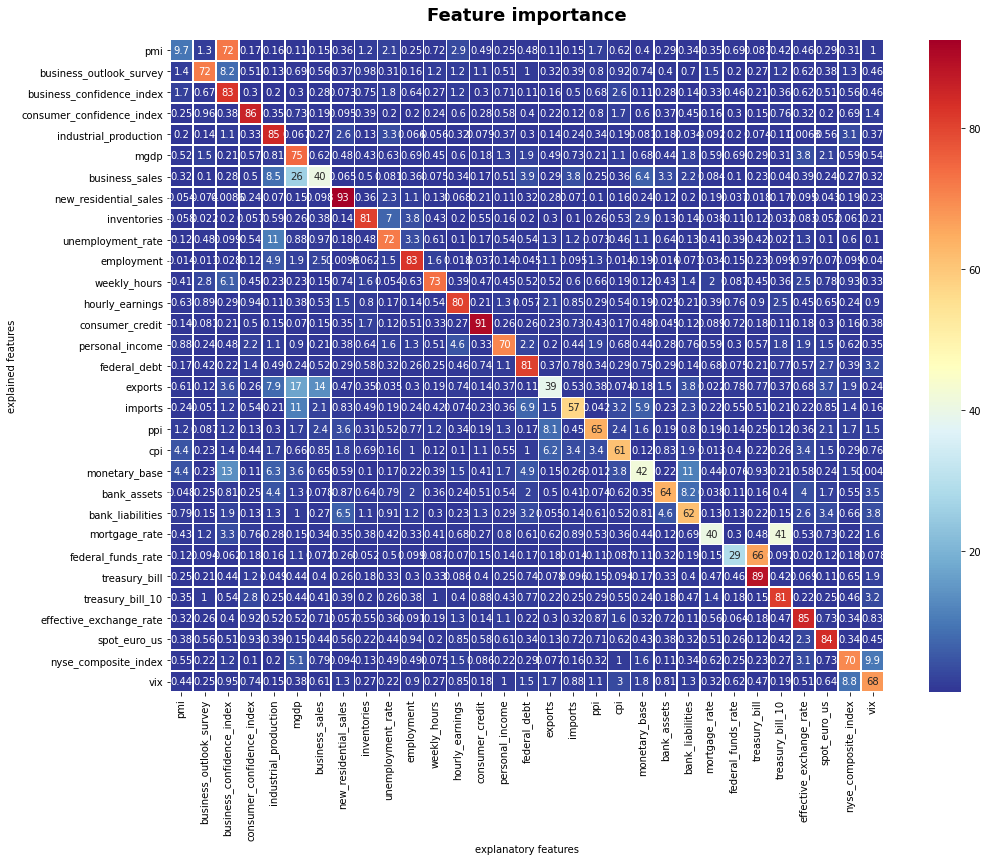
\includegraphics[scale=0.5]{images/variable_importance_others.png}
\caption{Variable importance for the dataset features}
\label{fig_c3_s8_ss4_2} \vspace{-5mm}
\end{figure}

A vast majority of features is determined primarily by its own lags, as one would expect, the other features individualy representing only a marginal fraction of the predictive capacity. Yet, a few features are interestingly enough determined by other features. This is the case for instance for: the pmi which is primarily determined by the business confidence index; the federal funds rate which is primarily determined by the treasury bill; and the mortgage rate which is determined at par by the 10-year treasury bill. In all these cases, there exist however solid theoretical connections between the features which explain the observed results.


\newpage























